\section*{HS11: Gömbalakú víztartály}
\addcontentsline{toc}{section}{Gömbalakú víztartály}

\begin{tabular}{ | p{2cm} | p{14cm} | } 
	\hline
	Név: & Drávai Tamás László GHKELE\\ 
	\hline
	Szak: & Mechatronikai mérnök \\ 
	\hline
	Félév: & 2019/2020 II. (tavaszi) félév \\ 
	\hline
\end{tabular}
\vspace{4mm}
%\\HS11 feladat:\\
\\Egy $\SI{1,5}{\meter} (R_1)$ sugarú gömb alakú víztartályt $\SI{0,15}{\meter}$ vastag($\delta$) üvegpaplan szigeteléssel láttak el. Számítsuk ki a tartályba óránként beáramló hőmennyiséget valamint azt, hogy a tartályban lévő víz hőmérséklete óránként mennyit emelkedik. A szigetelés külső felületének hőmérséklete $T_{sz}=\SI{50}{\celsius}$, míg a tartály belső felületének hőmérséklete $T_{b}=\SI{20}{\celsius}$ .
\subsection*{Adatok}
\begin{equation*}
\lambda=\SI[per-mode=fraction]{0,037}{\watt\per\meter\per\kelvin} \quad 
\varrho_{víz} =\SI[per-mode=fraction]{998,2}{\kilogram\per\cubic\meter}\quad 
c_{\textit{víz}}=\SI[per-mode=fraction]{4,118}{\kJ \per \kilogram\per\kelvin}\quad
\end{equation*}
\subsection*{Feladat megoldás}
Alap összefüggés felírása:
\begin{equation}
\dot{Q} =\dfrac{4 \pi  \lambda_{sz}}{\dfrac{1}{R_2} - \dfrac{1}{R_1}} (T_b-T_{sz}) 
\end{equation}
\begin{equation*}
R_2=R_1+\delta=\SI{1,5}{\meter}+\SI{0,15}{\meter}=\SI{1,65}{\meter}
\end{equation*}
Hőmérséklet értékek átváltása Kelvin skálára majd minden változót  behelyettesítünk az alap összefüggésbe 
\begin{equation}
\dot{Q}=\dfrac{4\pi\SI[per-mode=fraction]{0,037}{\watt\per\meter\per\kelvin}}
{\dfrac{1}{\SI{1,5}{\meter}}-\dfrac{1}{\SI{1,65}{\meter}}}
\hspace{1mm} (\SI{293,15}{\kelvin}-\SI{323,15}{\kelvin})
\end{equation}
A kapott hőmennyiség:
\begin{equation}
\dot{Q}=-230,153 W
\end{equation}
Átváltás $\SI[per-mode=fraction]{}{\J \per\hour}$-ra  azért, hogy meghatározzuk óránként mennyivel emelkedik a tartályban lévő víz hőmérséklete.
\begin{equation}
\SI[per-mode=fraction]{-230,153}{\J \per\second}=\SI[per-mode=fraction]{-230,153}{\J \per\second}\cdot 3600=\SI[per-mode=fraction]{-828551,01}{\J \per\hour}
\end{equation}
Víz hőmérséklet emelkedésének számítása:
Első lépésként a víztömeg kiszámítása sűrűség és térfogat alapján:
%\tudom, hogy nem kellene a \cdot de bántj a hiánya a szép érzetemet
\begin{equation}
m_{\textit{víz}}=\varrho_{\textit{víz}} V_{\textit{víz}}
\end{equation}
\begin{equation}
V_{\textit{víz}}=\dfrac{4\pi R^3_1}{3}=\dfrac{4\pi 1,5^3\SI{}{\cubic \meter} }{3}=\SI{14,137}{\cubic \meter}
\end{equation}
\begin{equation}
m_{\textit{víz}}=\SI[per-mode=fraction]{998,2}{\kilogram\per\cubic\meter}\SI{14,137}{\cubic \meter} =\SI{14111,72}{\kg}
\end{equation}
Minden adat birtokában kiszámolhatjuk a víz hőmérséklet emelkedését
\begin{equation}
\dfrac{dT}{dt}=\dfrac{\dot{Q}}{c_{\textit{víz}} \hspace{2mm} m_{\textit{víz}}}=
\dfrac{\SI[per-mode=fraction]{-828551,01}{\J \per\hour}}{\SI[per-mode=fraction]{4,118}{\kJ \per \kilogram\per\kelvin} \hspace{2mm} \SI{14111,72}{\kg}}
=\SI[per-mode=fraction]{-0,01425}{\kelvin \per\hour}
\end{equation}
Tehát a víz hőmérséklete az előjelet figyelembe véve azt mondhatjuk, hogy hűl óránként $\SI{0,01425}{\kelvin}$.
\begin{figure}[h]
	\centering
	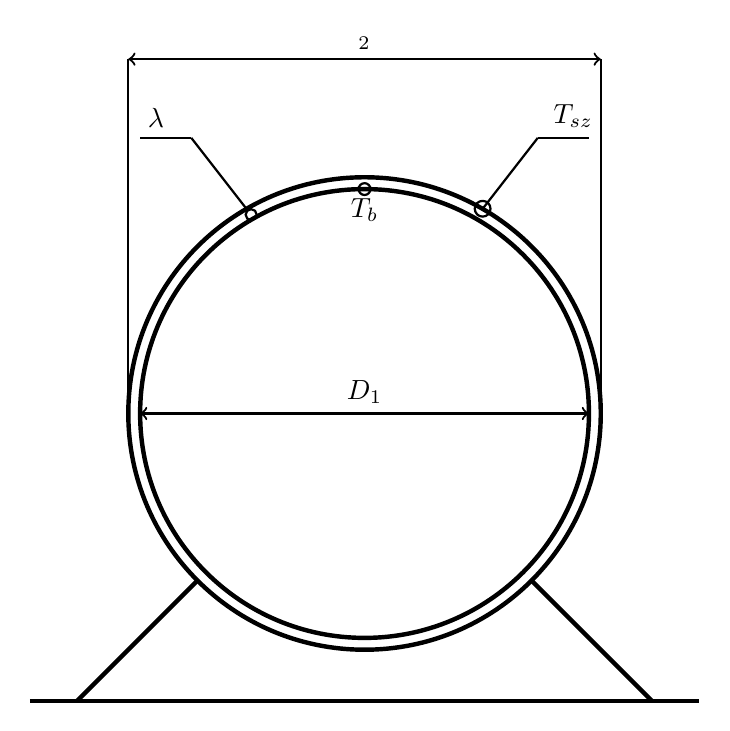
\begin{tikzpicture}
	%\draw[] (-6, -6) rectangle (6, 6);
	\draw[color =black, ultra thick] (0, 0) circle (30 mm); %külső fal	
	\draw[color =black,ultra thick] (0, 0) circle (2. 85) ;%belső fal 	
	\draw[thick,<->] (-2.85,0) -- (2.85,0);% méretnyíl
	\draw (0,0)  node[above] {$\diameter D_1  $};
	\draw[thick,<->] (-3,4.5) -- (3,4.5); %felső méretnyíl
	\draw (0,4.5)  node[above] {$ \diameterD_2  $};
	\draw [thick] (-3,0) -- (-3,4.5) (3,0) -- (3,4.5); %%felső méretnyíl oldalt
	\draw [ultra thick] (-2.13,-2.13) -- (-3.65,-3.65) (2.13,-2.13) -- (3.65,-3.65); %lábak
	\draw [ultra thick] (-4.25,-3.65) -- (4.25,-3.65) ;%földvonal
	%Tsz
	\draw [thick] (1.5,2.6) circle (0.1) (1.5,2.6) -- (2.2,3.5)  ;
	\draw [thick]  (2.2,3.5) -- (2.85,3.5) ;
	\draw [thick](2.65,3.5)  node[above] {$T_{sz}$};
	% lambda
	\draw [thick] (-1.44,2.525) circle (0.07) (-1.5,2.6) -- (-2.2,3.5)  ;
	\draw [thick]  (-2.2,3.5) -- (-2.85,3.5) ;
	\draw [thick](-2.65,3.5)  node[above] {$\lambda$};
	%T2
	\draw [thick] (0,2.85) circle (0.075) ;
	\draw (0,2.85)  node[below] {$T_b$};	
	\end{tikzpicture}
	\caption{ Gömb alakú főzőüst}
\end{figure}
\begin{figure}
	\centering
	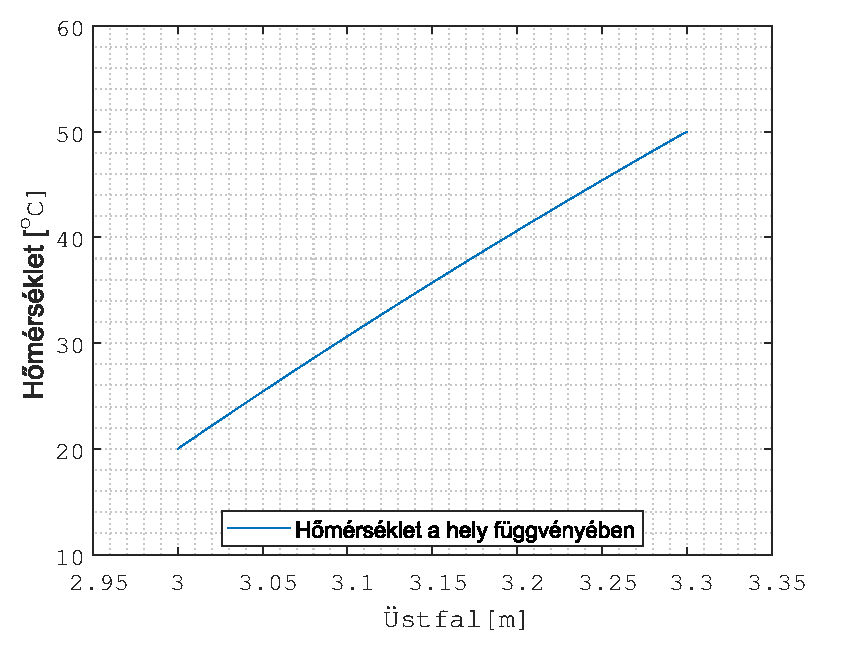
\includegraphics[width=1\linewidth]{./GHKELE/homersekletfuggvenyHS11}
	%dolgozok még rajta
	\caption{}
	\label{fig:waveforms}
\end{figure}
